\section{Experiments}
\label{sec:experiments}
We first establish the composition gap and identify evidence-access heads, then trace \emph{Locate--Route--Read} through address recovery, access interventions, and local-pattern transfer. Aggregate results and two concrete cases connect this mechanism to improved answers.

\subsection{Experimental Setup}
\label{sec:setup}
\textbf{Models and data.} We evaluate Qwen3-4B, Qwen3-8B \citep{yang2025qwen3}, and Llama-3.1-8B-Instruct \citep{grattafiori2024llama3} with native chat templates, BF16 computation, and greedy decoding; Qwen thinking mode is disabled. \dataset\ contains 100 discovery, 2,000 training, and 1,000 test sources with disjoint IDs. Each source retains ten paragraphs and three queries. Discovery selects heads and access targets; training fits head updates and address readers. The shared-context diagnostic uses 25 discovery quadruplets (Appendix~\ref{app:data}).

\textbf{Training and metrics.} Head adaptation and full fine-tuning use the same 2,000 composed examples, one epoch, AdamW \citep{loshchilov2019adamw}, learning rate $2\times10^{-5}$, and eight-example accumulation. Core QA uses normalized alias exact match with EOS completion within 32 tokens \citep{alab2020twikievaluation}. We report CFR, composed accuracy, and all-three accuracy (\cref{sec:triplets}). Adapted results are means and sample SDs over three recorded runs. Paired intervals resample test sources or, for factorial interventions, entire quadruplets. Appendix~\ref{app:protocol} specifies the prompts, scoring, and runs.

\subsection{Correct Hops, Failed Composition}
\label{sec:phenomenon}
\textbf{A gap under shared evidence.} The native models correctly answer both constituents on $457/462/501$ test sources. Approximately half of these sources still fail on composition: CFR is \scores{51.2}{51.1}{48.5}\% (\cref{fig:composition_gap}). The gap persists under permissive alias matching (Appendix~\ref{app:scoring_protocol}). We therefore examine how the composed query changes access to the same evidence.

\begin{figure}[!ht]
  \centering
  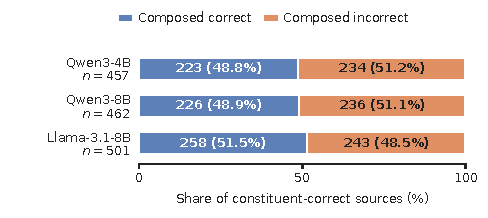
\includegraphics[width=\columnwidth]{figures/data_main_composition.pdf}
  \caption{\textbf{Correct constituent answers often fail to compose.} Native composed outcomes within each model's constituent-correct test population. Each bar conditions on correct answers to both constituent questions.}
  \label{fig:composition_gap}
\end{figure}

\textbf{A localized change in bridge access.} Paired direct--composed queries reveal a restricted band of high-scoring heads (\cref{fig:localization}). Layer-wise mean gaps peak near layers 20--24 in Qwen and 13--14 in Llama (\cref{fig:head_pair}a). These heads allocate more attention to the bridge when the question names it explicitly.

\begin{figure}[!ht]
  \centering
  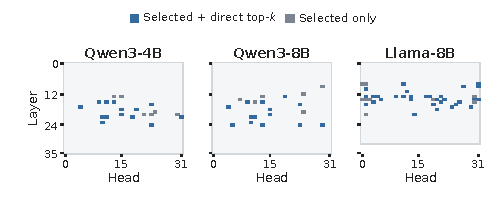
\includegraphics[width=\columnwidth]{figures/data_main_localization.pdf}
  \caption{\textbf{Bridge access changes in a localized set of heads.} Direct-minus-composed bridge attention for Qwen3-4B and Llama-3.1-8B (0.02-wide bins, shared scale). Boxes mark the selected heads; complete maps appear in \cref{fig:layer_profiles}.}
  \label{fig:localization}
\end{figure}

\textbf{The heads contribute causally to answering.} Knocking out the selected $20/20/40$ heads lowers composed accuracy to \scores{7.4}{5.5}{6.4}\%, compared with \scores{24.4}{27.3}{29.4}\% after layer-matched random knockout. The dose curves separate as more heads are removed (\cref{fig:head_pair}b). Constituent-query effects (\cref{fig:necessity}) connect this contribution to evidence access across query formulations.

\begin{figure}[!ht]
  \centering
  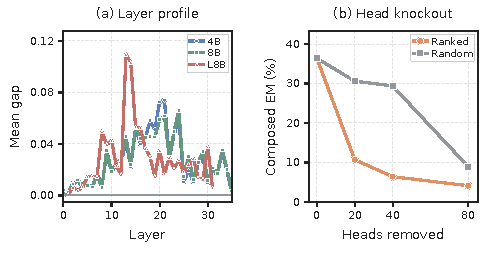
\includegraphics[width=\columnwidth]{figures/data_main_head_pair.pdf}
  \caption{\textbf{Evidence-access heads affect the answer computation.} (a) Layer-wise mean direct-minus-composed bridge attention. (b) Llama composed accuracy under ranked versus layer-matched random knockout. Lines connect measured doses. 4B/8B: Qwen3; L8B: Llama-3.1-8B.}
  \label{fig:head_pair}
\end{figure}

\subsection{Locate: Bridge Addresses Survive Failure}
\label{sec:address_results}
The first operation locates the next fact. On the native composition failures above, the training-fitted readout recovers the bridge paragraph in $169/234$, $176/236$, and $209/243$ cases: \scores{72.2}{74.6}{86.0}\% (\cref{fig:diagnosis}). Many wrong answers therefore coexist with a recoverable address.

\begin{figure}[!ht]
  \centering
  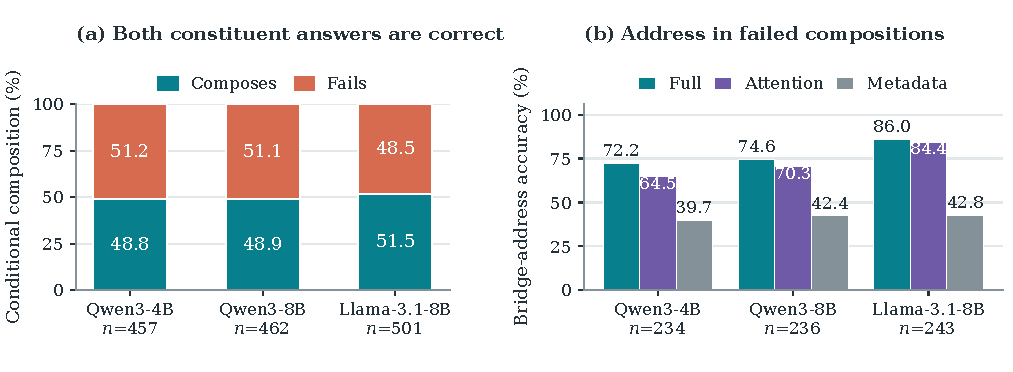
\includegraphics[width=\columnwidth]{figures/data_fig3_diagnosis.pdf}
  \caption{\textbf{Locate: bridge addresses remain recoverable during failure.} Reader accuracy on the 234/236/243 native failures with correct constituents. Attention features carry location information beyond length and title-mention metadata.}
  \label{fig:diagnosis}
\end{figure}

Attention-only readers reach \scores{64.5}{70.3}{84.4}\%, versus \scores{39.7}{42.4}{42.8}\% from metadata alone. This establishes an address signal in the selected heads and motivates asking how attention is routed to that address.

\subsection{Route: Access Has a Specific Destination}
\label{sec:routing_results}
Calibrating bridge attention mass improves composed accuracy by \scores{4.9}{5.5}{16.0} percentage points on the 1,000 test questions (\cref{fig:access_controls}). The same targets applied to the root or a length-matched other paragraph do not yield this gain. Routing therefore depends on \emph{where} access is allocated. We next examine how it changes the use of tokens within that destination.

\begin{figure}[!ht]
  \centering
  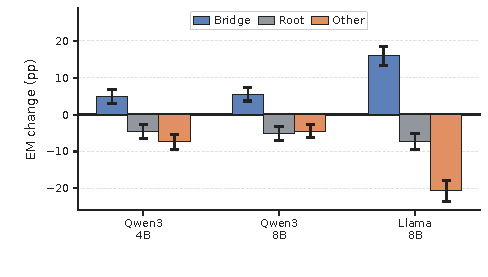
\includegraphics[width=\columnwidth]{figures/data_app_access_controls.pdf}
  \caption{\textbf{Route: the destination of access matters.} Composed-accuracy changes when identical frozen mass targets are assigned to the bridge, root, or a length-matched other paragraph. Error bars: paired 95\% intervals over 1,000 test sources.}
  \label{fig:access_controls}
\end{figure}

\subsection{Read: Local Patterns Depend on Routing}
\label{sec:causal_results}
\textbf{The same reading pattern has different effects.} \Cref{fig:causal} crosses access mass and local token weighting under shared evidence. For Llama, Native/Mass/Pattern/Both reach 51/64/47/76\% accuracy. Transferring the direct-query pattern changes accuracy by $-4$ points under native access and by $+12$ points after calibration. Its usefulness changes even though the transferred pattern is identical.

\begin{figure*}[!t]
  \centering
  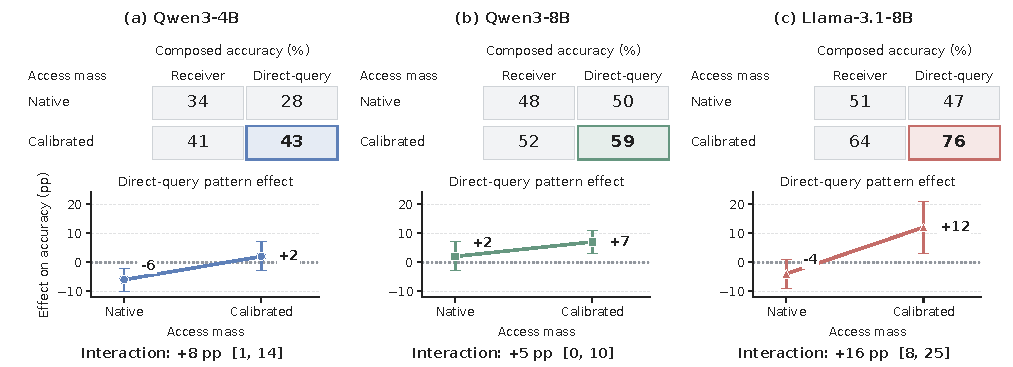
\includegraphics[width=\textwidth]{figures/data_main_causal_pair.pdf}
  \caption{\textbf{Read: routing changes the utility of local token weighting.} Upper: composed accuracy (\%) for native/calibrated bridge mass and receiver/direct-query patterns. Lower: the pattern-transfer effect at each mass; their difference is the interaction. Error bars and interaction intervals are paired 95\% quadruplet-bootstrap intervals over 100 receivers in 25 discovery quadruplets.}
  \label{fig:causal}
\end{figure*}

Qwen shows the same direction of interaction: pattern effects change from $-6/+2$ points under native access to $+2/+7$ after calibration. The interaction estimates are \scores{8}{5}{16} points, with 95\% intervals $[1,14]$, $[0,10]$, and $[8,25]$ (\cref{tab:factorial}). For Llama, the separate effects predict $64+47-51=60\%$ accuracy additively, while Both reaches 76\%. Successful reading depends on the coordination of paragraph access and local weighting.

\subsection{From Mechanism to Evidence-Sensitive Repair}
\label{sec:repair_results}
\textbf{Improving complete compositions.} \method\ uses the recovered addresses to select evidence and adapts the localized heads. Composed EM rises from \scores{26.9}{29.2}{36.4}\% to \scores{66.8}{67.2}{69.7}\%, gains of \scores{39.9}{38.0}{33.3} points (\cref{tab:main}). All-three accuracy improves from \scores{22.3}{22.6}{25.8}\% to \scores{41.3}{45.4}{42.3}\%.

\begin{table*}[!t]
  \centering
  \caption{\textbf{Mechanism-guided repair improves contextual composition.} Completed-answer EM (\%) on 1,000 test sources. All three requires correct constituent and composed answers. Trained configurations share the same 2,000 composed training examples. Values are mean $\pm$ sample SD over three recorded runs; Native is measured once.}
  \label{tab:main}
  \small\setlength{\tabcolsep}{3.3pt}
  % Generated by analysis/build_tables.py.
\begingroup\renewcommand{\arraystretch}{1.08}
\begin{tabular}{lrrrrrr}
\toprule
 & \multicolumn{2}{c}{\textbf{Qwen3-4B}} & \multicolumn{2}{c}{\textbf{Qwen3-8B}} & \multicolumn{2}{c}{\textbf{Llama-3.1-8B}} \\
\cmidrule(lr){2-3}\cmidrule(lr){4-5}\cmidrule(lr){6-7}
\textbf{Method} & \textbf{Composed $\uparrow$} & \textbf{All three $\uparrow$} & \textbf{Composed $\uparrow$} & \textbf{All three $\uparrow$} & \textbf{Composed $\uparrow$} & \textbf{All three $\uparrow$} \\
\midrule
\multicolumn{7}{l}{\textit{Baselines}} \\
Native & $26.9$ & $22.3$ & $29.2$ & $22.6$ & $36.4$ & $25.8$ \\
Evidence selection & $47.2{\color{black!80}\,\pm\,0.1}$ & $33.1{\color{black!80}\,\pm\,0.1}$ & $48.1{\color{black!80}\,\pm\,0.0}$ & $33.8{\color{black!80}\,\pm\,0.0}$ & $53.4{\color{black!80}\,\pm\,0.1}$ & $39.5{\color{black!80}\,\pm\,0.1}$ \\
Full fine-tuning & $57.1{\color{black!80}\,\pm\,2.4}$ & $17.4{\color{black!80}\,\pm\,2.2}$ & $55.2{\color{black!80}\,\pm\,5.3}$ & $14.1{\color{black!80}\,\pm\,5.8}$ & $35.2{\color{black!80}\,\pm\,3.4}$ & $3.6{\color{black!80}\,\pm\,0.7}$ \\
\midrule
\multicolumn{7}{l}{\textit{Mechanistically-Informed Head-Tuning (Ours)}} \\
Head adaptation & $60.1{\color{black!80}\,\pm\,0.1}$ & $39.4{\color{black!80}\,\pm\,0.0}$ & $61.8{\color{black!80}\,\pm\,0.0}$ & $41.6{\color{black!80}\,\pm\,0.0}$ & $63.6{\color{black!80}\,\pm\,0.2}$ & $25.0{\color{black!80}\,\pm\,0.1}$ \\
\textbf{\method} & $\mathbf{66.8}{\color{black!80}\,\pm\,0.3}$ & $\mathbf{41.3}{\color{black!80}\,\pm\,0.1}$ & $\mathbf{67.2}{\color{black!80}\,\pm\,0.0}$ & $\mathbf{45.4}{\color{black!80}\,\pm\,0.0}$ & $\mathbf{69.7}{\color{black!80}\,\pm\,0.2}$ & $\mathbf{42.3}{\color{black!80}\,\pm\,0.0}$ \\
\textit{Gain over Native (pp)} & {\color{gain}$+39.9$} & {\color{gain}$+19.0$} & {\color{gain}$+38.0$} & {\color{gain}$+22.8$} & {\color{gain}$+33.3$} & {\color{gain}$+16.5$} \\
\bottomrule
\end{tabular}
\endgroup

\end{table*}

On the fixed native constituent-correct population, \method\ repairs \scores{80.8}{80.9}{77.8}\% of composition failures and retains \scores{94.6}{92.9}{95.1}\% of composed successes (\cref{tab:fixed_population}). Full fine-tuning reaches \scores{57.1}{55.2}{35.2}\% composed EM under the same training recipe. Selected Q/K/V/O slices comprise \scores{0.59}{0.49}{0.94}\% of model parameters; readers add $42/42/82$ weights. Evidence selection reduces composed-generation input tokens by 56.3--57.6\%, with an extra reader prefill on 10.3\% of inputs. Appendices~\ref{app:application}--\ref{app:efficiency} report components, capabilities, and workload.

\textbf{Following local fact changes.}
\label{sec:content_results}
We reciprocally exchange object spans between bridge paragraphs expressing the same relation. Questions, titles, order, and full-context word and character multisets remain fixed while the correct answer changes. Applying the complete procedure, including evidence selection, to the 100 exchanges yields \scores{77}{76}{80}\% edited-value accuracy, versus Native \scores{26}{35}{32}\%. Joint original/edited correctness rises from \scores{21}{29}{29}\% to \scores{75}{72}{77}\% (\cref{fig:content}). The repaired answers follow the local relation values.

\begin{figure}[!ht]
  \centering
  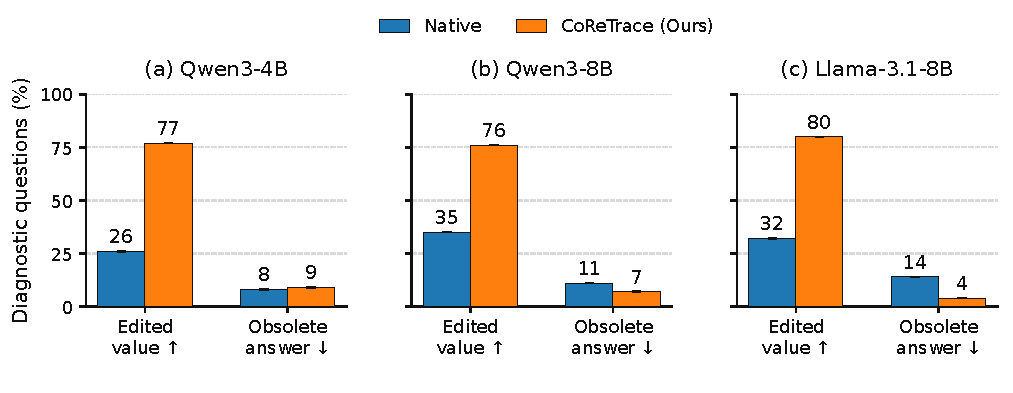
\includegraphics[width=\columnwidth]{figures/data_fig5_content.pdf}
  \caption{\textbf{Repaired answers track changed local values.} Edited-value accuracy and joint original/edited correctness on the 100 reciprocal exchanges from the 25 discovery quadruplets.}
  \label{fig:content}
\end{figure}

\clearpage
\twocolumn[{
\begin{minipage}{\textwidth}
\centering
\captionsetup{hypcap=false}
  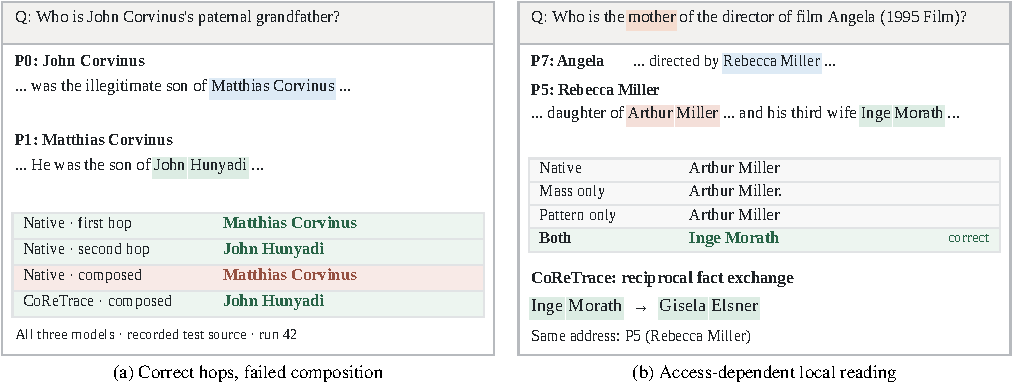
\includegraphics[width=\textwidth]{figures/data_main_mechanism_cases.pdf}
  \captionof{figure}{\textbf{Two cases connect evidence location, routing, and relation reading.} (a) All three models answer both constituents correctly but repeat the bridge entity on a test composition; \method\ reaches the endpoint. (b) On a shared-context Llama diagnostic, joint mass and pattern intervention yields the requested mother. The complete \method\ procedure also follows the reciprocal change in her name. Text and answers come from recorded contexts and predictions.}
  \label{fig:mechanism_cases}
\end{minipage}
\vspace{1em}
}]

\subsection{Case Study: From an Address to the Right Fact}
\label{sec:cases}
\Cref{fig:mechanism_cases} makes the three operations concrete. In the John Corvinus test case, all three native models correctly identify Matthias Corvinus as the father and John Hunyadi as Matthias's father, yet return Matthias for the composed question. \method\ selects the bridge paragraph and answers John Hunyadi. The example exposes the distinction between identifying the intermediate entity and reading the next relation.

The Angela case shows why routing and reading must work together. Asked for the director's mother, Llama returns Arthur Miller under Native, Mass, and Pattern, but Inge Morath under Both. On the same shared context, \method\ answers Inge Morath and then Gisela Elsner after their reciprocal exchange, while retaining the selected bridge paragraph. The address stays fixed; the answer changes with the relation's local value.
